\documentclass[aspectratio=169,10pt,dvipsnames,handout]{beamer}

%\setbeameroption{show notes}

\input{preamble.inc}

\title{Introduzione alla logica dei predicati}

\begin{document}

\begin{frame}
	\titlepage
\end{frame}

\begin{frame}
	\copyrightpage
\end{frame}

\begin{frame}
	\bookpage{sulle sezioni da 1.1 a 1.4}
\end{frame}

\begin{frame}{Inferenze a livello predicativo}
	Fino ad ora abbiamo trattato la \emph{logica proposizionale}. Nella logica proposizionale il costrutto di base è la proposizione, e proposizioni più complesse si ottengono tramite connettivi logici.

	\medskip
	Quando entrano in gioco i \emph{quantificatori}, la logica proposizionale non è più sufficiente per determinare la validità di una inferenza.

	\begin{center}
		\begin{inference}
			Napoleone è corso\\
			Tutti i corsi sono francesi\\
			\hline
			Napoleone è francese
		\end{inference}
		\qquad
		\begin{inference}
			Socrate è un uomo\\
			Tutti gli uomini sono mortali\\
			\hline
			Socrate è mortale
		\end{inference}
	\end{center}
	Se analizzate come fatto fin'ora, corrispondo alla regola di inferenza:
	\begin{center}
		\begin{inference}
			A\\
			B\\
			\hline
			C
		\end{inference}
	\end{center}
	che non è corretta! Bisogna passare alla \alert{logica dei predicati} e iniziare ad indagare la \alert{struttura delle proposizioni semplici}.
\end{frame}

\section{Proposizioni semplici del 1° tipo e del 2° tipo}

\begin{frame}{Proposizioni semplici del primo tipo (1)}
	Consideriamo queste proposizioni semplici:
	\begin{center}
		\propshape
		Stefano {\only<2->{\color{brown}}è italiano}\\
		Marco {\only<2->{\color{brown}}sta leggendo}\\
		Carlo {\only<3->{\color{green}}è più alto di} Massimo\\
		Monza {\only<3->{\color{green}}ha più abitanti} di Milano\\
		Dario {\only<4->{\color{blue}}è figlio di} Ernesto {\only<4->{\color{blue}}e} Maria\\
		Marcello {\only<4->{\color{blue}}va a} Torino {\only<4->{\color{blue}}con}  Claudia
	\end{center}
	In queste proposizioni interviene:
	\begin{itemize}
		\item<2-> una \textcolor{brown}{proprietà} \tikz[remember picture] \node (i1) {};
		\item<3-> una \textcolor{green}{relazione binaria} \tikz[remember picture] \node (i2) {};
		\item<4-> una \textcolor{blue}{relazione ternaria} \tikz[remember picture] \node (i3) {};
		\item<5-> in generale, una relazione $n$-aria \tikz[remember picture] \node (i4) {};
	\end{itemize}
	\visible<6->{\begin{tikzpicture}[remember picture, overlay]
			\node (p) [right=4cm of i2] {\alert{predicati}};
			\draw [->,red] (i1) edge (p);
			\draw [->,red] (i2) edge (p);
			\draw [->,red] (i3) edge (p);
			\draw [->,red] (i4) edge (p);
		\end{tikzpicture}}
\end{frame}

\begin{frame}{Proposizioni semplici del primo tipo (2)}
	\begin{definition}[Proposizioni semplici del 1° tipo]
		Le \alert{proposizioni semplici del 1° tipo}, dette anhe \alert{proposizioni atomiche}, sono proposizioni in cui un predicato ad $n$ argomenti viene applicato ad $n$ individui.
	\end{definition}

	\medskip
	Cosa sia un \emph{individuo} dipende dal contesto: persone, numeri, città, pianeti, etc\ldots

	\medskip
	In realtà, quella di \emph{proposizione semplice del 1° tipo} è la terminologia usata dal libro di testo, ma il termine di \emph{proposizione atomica} è molto più standard.
\end{frame}

\begin{frame}{Nomi e descrizioni definite}
	Ci si può riferire ad un individuo in vari modi:
	\begin{itemize}
		\item tramite un \alert{nome proprio}: Carlo, 13, Giove
		\item tramite una \alert{descrizione definita} che comunque lo identifica in maniera univoca: il fratello di Michele, 15-2, il pianeta più grande del sistema solare
	\end{itemize}

	\pause
	\begin{example}[Esempi di proposizioni con descrizioni definite]
		\centering
		\propshape
		\alert{Il cane di Giovanni} è fedele\\
		\alert{Il figlio di Aldo} ha sposato \alert{la sorella di Giuseppe}\\
		\alert{$5^2+3$} è pari
	\end{example}

	\pause
	\medskip
	Con la parola \alert{termine} si indica o un nome proprio o una descrizione definita.
\end{frame}

\begin{frame}{Individui e termini}
	C'è una differenza tra termine ed individuo, simile alla differenza tra \emph{proposizione} ed \emph{enunciato}:
	\begin{itemize}
		\item Un \emph{individuo} è una entita che appare in una proposizione;
		\item Un \emph{termine} è una espressione linguistica che indica un individuo.
	\end{itemize}

	\medskip
	Ad esempio,
	\begin{itemize}
		\item \alert{Giove}
		\item \alert{il pianeta più grande del sistema solare}
	\end{itemize}
	sono due termini che denotano lo stesso individuo.
\end{frame}

\begin{frame}{Proposizioni semplici del 2° tipo}
	Consideriamo ora queste proposizioni semplici:
	\begin{center}
		\propshape
		Tutti gli uomini sono mortali\\
		Vi è un italiano più alto di due metri\\
		Ogni studente universitario frequenta almeno un corso
	\end{center}
	Iniziano con dei \alert{quantificatori}: \quant{tutti}, \quant{ogni}, \quant{vi è}, \quant{almeno}.

	\pause
	\medskip
	\begin{definition}[Proposizioni semplici del 2° tipo]
		Le \alert{proposizioni semplici del 2° tipo} sono le proposizioni che iniziano con un quantificatore.
	\end{definition}

	\pause
	\medskip
	Anche la terminologia di \emph{proposizione semplice del 2° tipo}, come quella di \emph{proposizione semplice del 1° tipo} è specifica del libro di testo e non molto utilizzata in generale.
\end{frame}

\section{Quantificatori}

\begin{frame}{Universo del discorso}
	Quando si utilizzano dei quantificatori è sempre implicito un \alert{universo del discorso}, detto anche \alert{dominio di quantificazione}, che è l'insieme di tutti gli individui su cui stiamo quantificando.

	\medskip
	Ad esempio, consideriamo le proposizioni
	\begin{center}
		\propshape
		Tutti hanno passato l'esame\\
		Qualcuno ha passato l'esame
	\end{center}

	\smallskip
	Chi sono questi ``\quant{tutti}'' ?\\
	Da quale insieme possiamo scegliere questo ``\quant{qualcuno}'' che ha passato l'esame ?\\

	\smallskip
	Si parla probabilmente di una classe di una scuola, che costituisce l'univero del discorso.
\end{frame}

\begin{frame}{Quantificatori limitati e illimitati}
	Consideriamo le proposizioni:
	\begin{center}
		\propshape
		Tutti hanno passato l'esame.\\
		Tutti i pendolari hanno passato l'esame.
	\end{center}

	\medskip
	Nel primo caso stiamo affermando che tutti gli individui che fanno parte dell'universo del discorso hanno passato l'esame. Si parla di \alert{quantificatore illimitato}.

	\medskip
	Nel secondo caso, il quantificatore si applica solo ad una parte degli individui, quelli che sono pendolari. Sugli individui non pendolari non ci esprimiamo (potrebbero aver passato l'esame tutti, non averlo passato nessuno, oppure alcuni sì e altri no.). Si parla di \alert{quantificatore limitato}.

	\medskip
	Vedere anche la differenza tra
	\begin{center}
		\propshape
		Qualcuno ha passato l'esame.\\
		Qualche pendolare ha passato l'esame.
	\end{center}
\end{frame}

\begin{frame}{I quantificatori ``per ogni'' ed ``esiste''}
	Esistono molti quantificatori: tutti, qualcuno, ciascuno, qualcheduno, vi è, ogni, etc\ldots, sia limitati che illimitati. In realtà, ne bastano due, i quantificatori illimitati ``per ogni x'' ed  ``esiste x tale che''.
	\begin{itemize}
		\item \alert{per ogni}, chiamato \alert{quantificatore universale}, che equivale a \quant{tutti}, \quant{ogni}, etc..\\[0.1cm]
		      \quad ``\prop{per ogni $x$, \ldots}'' significa: tutti gli individui soddisfano \ldots
		\item \alert{esiste}, chiamato \alert{quantificatore esistenziale}, che equivale a \quant{vi è}, \quant{almeno}, etc..\\[0.1cm]
		      \quad ``\prop{esiste x tale che \ldots}'' significa: vi è almeno un individuo che soddisfa \ldots
	\end{itemize}

	\medskip
	Le proposizioni semplici che iniziano con ``\quant{per ogni}'' si dicono \alert{quantificate universalmente}, quelle che iniziano con ``\quant{esiste}'' si dicono \alert{quantificate esistenzialmente}.

	\medskip
	L'uso di questi due quantificatori richiede l'introduzione di lettere come $x$, $y$, $z$, \ldots, chiamate \alert{variabili individuali}.
\end{frame}


\begin{frame}{Uso di ``per ogni'' ed ``esiste'' (1)}
	La maggior parte dei quantificatori possono essere rimpiazzati da \quant{per ogni} ed \quant{esiste}.

	\medskip
	\textbf{Quantificatori illimitati}:

	\smallskip
	\begin{tabular}{rcl}
		\prop{Tutti sono mortali}      & $\Rightarrow$ & \prop{Per ogni $x$, $x$ è mortale}           \\
		\prop{Vi è almeno un elefante} & $\Rightarrow$ & \prop{Esiste $x$ tale che $x$ è un elefante} \\
	\end{tabular}

	\medskip
	\textbf{Quantificatori illimitati}:

	\smallskip
	\begin{tabular}{rcl}
		\prop{Tutti gli uomini sono mortali}         & $\Rightarrow$ & \prop{Per ogni $x$, se $x$ è un uomo, allora $x$ è mortale}              \\
		\prop{C'è un italiano più alto di due metri} & $\Rightarrow$ & \prop{Esiste $x$ tale che $x$ è italiano ed $x$ è alto più di due metri}
	\end{tabular}

	\medskip
	\textbf{Quantificatori multipli}:

	\smallskip
	\begin{tabular}{l}
		\prop{Ogni studente universitario frequenta almeno un corso} \\
		\hspace{5cm} $\Downarrow$                                    \\
		\prop{Per ogni $x$, se $x$ è uno studente universitario, allora esiste $y$ tale che $y$ è un corso ed $x$ frequenta $y$}
	\end{tabular}
\end{frame}


\begin{frame}{Uso di ``per ogni'' ed ``esiste'' (2)}
	L'uso dei quantificatori \quant{per ogni} ed \quant{esiste} rende esplicito il ruolo e la presenza dei quantificatori nel linguaggio naturale.

	\begin{example}[Esempio]
		La proposizione

			{\medskip \propshape
				\quad Per ogni $x$, se $x$ è un uomo, allora $x$ è mortale.
			}

		\medskip
		corrisponde a
		\begin{itemize}
			\item \prop{Tutti gli uomini sono mortali}
			\item \prop{Ogni uomo è mortale}
			\item \prop{Qualunque uomo è mortale}
			\item \prop{Ciascun uomo è mortale}
		\end{itemize}
	\end{example}
\end{frame}



\begin{frame}{Quantificatori impliciti, vaghi e ambigui}
	\begin{enumerate}
		\item Nella lingua comune i quantificatori possono essere \alert{impliciti}:

		      \medskip
		      \begin{proposition}
			      Gli uomini sono mortali\\
			      L'uomo è mortale
		      \end{proposition}
		      Entrambi sono modi compatti di dire
		      \begin{proposition}
			      Tutti gli uomini sono mortali
		      \end{proposition}

		      \medskip\pause


		\item Nella lingua comune vi sono alcuni quantificatori \alert{vaghi} di cui non ci occupiamo:

		      \medskip
		      \begin{center}
			      \propshape
			      \quant{Quasi tutti} gli italiani sanno chi è il presidente della Repubblica.\\
			      \quant{La maggior parte dei} nordici ha i capelli biondi.
		      \end{center}
		      \medskip\pause

		\item Alcuni quantificatori nella lingua italiana sono \alert{ambigui}.	Ad esempio:

		      \medskip
		      \begin{center}
			      \propshape
			      Se \textcolor{orange}{qualcuno} è buono, allora \quant{qualcuno} lo ama.\\
			      $\Downarrow$\\
			      \textcolor{orange}{Per ogni $x$}, se $x$ è buono \quant{esiste $y$} tale che $y$ ama $x$.
		      \end{center}
		      \medskip

		      La stessa parola ``\quant{qualcuno}'' gioca  due ruoli differenti da quantificatore esistenziale ed universale.
	\end{enumerate}
\end{frame}

\note{Esercizi 1.5, 1.4 , 1.7}

\section{Variabili libere e vincolate}

\begin{frame}{Funzioni proposizionali e variabili libere}
	Analizziamo la proposizione ``{\propshape Per ogni $x$, se $x$ è un uomo, allora $x$ è mortale}''.

	\medskip
	\only<1|handout:0>{La frase ``{\propshape $x$ è un uomo}'' è una proposizione?}
	\only<2>{La frase ``{\propshape $x$ è un uomo}'' si chiama \alert{funzione proposizionale}. Non è una proposizione perché il valore di verità dipende da chi è $x$. Il libro li chiama anche \alert{predicati}.}

	\pause
	\medskip
	Dalla funzione proposizionale ``{\propshape $x$ e $y$ vanno a vedere $z$}'', possiamo ottenere altre funzioni proposizionali rimpiazzando le variabili con termini:
	\begin{itemize}
		\item {\propshape Stefano e $y$ vanno a vedere $z$}
		\item {\propshape Stefano e $y$ vanno a vedere il derby Milan-Inter}
		\item {\propshape Stefano e Marcello vanno a vedere $z$}
		\item \ldots
	\end{itemize}
	Se rimpiazzo tutte le variabili ottengo una proposizione:
	\begin{itemize}
		\item {\propshape Stefano e Marcello vanno a vedere  il derby Milan-Inter}
	\end{itemize}
	Si dice che le variabili $x$, $y$ e $z$, nei casi di sopra, sono \alert{libere}.
\end{frame}

\begin{frame}{Variabili vincolate}
	Le funzioni proposizionali possono essere trasformate in proposizioni:
	\begin{itemize}
		\item rimpiazzando variabili con termini (slide precedente);
		\item oppure, usando i quantificatori.
	\end{itemize}
	Per esempio, da  ``\prop{$x$ ama $y$}\/'' otteniamo:
	{\propshape
	\begin{itemize}
		\item \propshape Elisa ama Massimo\\
		\item Esiste $x$ tale che $x$ ama Massimo (Vi è qualcuno che ama Massimo)\\
		\item Per ogni $x$, $x$ ama Massimo (Tutti amano Massimo)\\
		\item Per ogni $y$, Elisa ama $y$ (Elisa ama tutti).
	\end{itemize}
	}
	In queste frasi, non si può rimpiazzare una variabile con un nome\ldots la frase seguente non ha alcun significato:
	\begin{itemize}
		\item {\propshape Esiste Elena tale che Elena ama Massimo}\\
	\end{itemize}
	Le variabili in questo caso si dicono \alert{vincolate}. I quantificatori \alert{vincolano} le variabili a cui sono applicate.
\end{frame}

\begin{frame}{Variabili libere e vincolate in matematica}
	Il concetto di variabile libera e vincolata non appare solo nella logica, ma anche in altre branche della matematica.

	\medskip Consideriamo ad esempio la formula
	\[
		\sum_{i=1}^{10} ij
	\]
	In questa formula, l'operazione di sommatoria svolge lo stesso ruolo del quantificatore, vincolando la variabile $i$. La variabile $j$ è invece libera.

	\medskip
	A causa di ciò, il risultato della sommatoria dipende solo dal valore di $j$: se eliminiamo la sommatoria svolgendo il calcolo, otteniamo la formula $55 j$ dove compare solo la variabile $j$.

	\medskip
	Come esempio finale, anche l'operazione di integrale definisce una variabile vincolata. Ad esempio, nell'integrale
	\[
		\int_0^1 x^2 \, dx
	\]
	$x$ è una variabile vincolata.
\end{frame}

\note{Esercizio 1.8}

\begin{frame}{Termini aperti (1)}
	Le variabili individuali possono anche apparire all'interno di un termine. Si parla di \alert{termini aperti}, mentre i termini senza variabili si chiamano più propriamente \alert{chiusi}.
	\begin{example}[Termini aperti]
		La frase ``{\propshape L'autore di $x$}'' è un termine aperto. Sostituendo $x$ con un altro termine si ottengono le descrizioni definite:
		\begin{itemize}
			\propshape
			\item L'autore della Divina Commedia\\
			\item L'autore della prima storia presente in Topolino n. 1374
		\end{itemize}
	\end{example}
	I termini aperti sono molto usati in matematica in maniera esplicita: $x+1$, $2x+5$, sono tutti termini  aperti.
\end{frame}

\begin{frame}{Termini aperti (2)}
	Nel linguaggio comune i termini aperti, come più in generale le variabili
	\begin{itemize}
		\item non compaiono mai esplicitamente;
		\item sono nascosti dalla presenza di pronomi.
	\end{itemize}

	\medskip
	Compaiono non appena riscriviamo le proposizioni usando i quantificatori \quant{per ogni} ed \quant{esiste \ldots tale che}.
	\begin{example}
		\propshape\centering
		Esiste un libro il cui autore è nato nel 1920.\\
		$\Downarrow$\\
		Esiste $x$ tale che l'autore di $x$ è nato nel 1920.
	\end{example}
\end{frame}


\begin{frame}{Termini e predicati}
	Volendo si può fare a meno di termini aperti e descrizioni definite, rimpiazzandoli con opportuni predicati. Più o meno l'idea è la seguente:

	\pause
	\begin{example}[Da descrizioni definite a predicati]
		\propshape\centering
		\alert{L'autore della Divina Commedia} è fiorentino\\
		$\Downarrow$\\
		Esiste $x$ tale che \alert{$x$ è autore della Divina Commedia} ed $x$ è fiorentino
	\end{example}

	Nell'esempio precedente ho rimpiazzato la descrizione definita ``autore della divina commedia'' con
	il predicato ``essere autore della divina commedia''. Analogamente:

	\pause
	\begin{example}[Da termini aperti a predicati]
		\propshape\centering
		\alert{L'autore di $y$} è fiorentino\\
		$\Downarrow$\\
		Esiste $x$ tale che \alert{$x$ è autore di $y$} ed $x$ è fiorentino
	\end{example}

\end{frame}

\section{Valore di verità di una proposizione}

\begin{frame}{Valore di verità di una proposizione}
	Nella logica proposizionale, per stabilire il valore di verità di una proposizione è sufficiente essere in grado di stabilire il valore di verità delle proposizioni semplici, e applicare le regole dei connettivi.

	\pause\medskip
	Nella logica dei predicati dobbiamo:
	\begin{itemize}
		\item stabilire il valore di verità delle proposizioni atomiche;
		\item applicare le regole dei connettivi;
		\item applicare le regole dei quantificatori.
	\end{itemize}

	\pause\medskip
	Vedremo ora questo aspetto in maniera informale e rimandiamo un trattamento più formale ad una lezione successiva.
\end{frame}

\begin{frame}{Il quantificatore universale (1)}
	Consideriamo la seguente proposizione:
	\begin{proposition}
		Tutte le vocali compaiono nella parola ``aiuole''.
	\end{proposition}
	Come facciamo ad affermare che questa proposizione è vera o falsa? Prima di tutto, rimpiazziamo il quantificatore \quant{tutti} con \quant{per ogni}, ottenendo:
	\begin{proposition}
		Per ogni $x$, se $x$ è una vocale allora $x$ compare nella parola ``aiuole''.
	\end{proposition}

	\medskip
	Ora dovremmo capire dal contesto qual è l'\emph{universo del discorso}. Sembra ragionevole assumere che sia l'insieme delle lettere dell'alfabeto italiano.

	\medskip La proposizione
	\begin{proposition}
		Per ogni $x$, se $x$ è una vocale allora $x$ compare nella parola ``aiuole''
	\end{proposition}
	quando rimpiazzo $x$ con una lettera in \prop{e $x$ è una vocale allora $x$ compare nella parola ``aiuole''} ottengo sempre una proposizione vera.
\end{frame}

\begin{frame}{Il quantificatore universale (2)}
	In altri termini, la proposizione
	\begin{center}
		\propshape
		Per ogni $x$, se $x$ è una vocale allora $x$ compare nella parola ``aiuole''.
	\end{center}
	è vera quando tutte le seguenti proposizioni sono vere:
	\begin{itemize}
		\item $x \mapsto a$: \prop{se la lettera ``a'' è una vocale allora ``a'' compare nella parola ``aiuole''}
		\item $x \mapsto b$: \prop{se la lettera ``b'' è una vocale allora ``b'' compare nella parola ``aiuole''}
		\item $x \mapsto c$: \prop{se la lettera ``c'' è una vocale allora ``c'' compare nella parola ``aiuole''}
		\item \ldots
		\item $x \mapsto l$: \prop{se la lettera ``l'' è una vocale allora ``l'' compare nella parola ``aiuole''}
		\item \ldots
		\item $x \mapsto z$: \prop{se la lettera ``z'' è una vocale allora ``z'' compare nella parola ``aiuole''}
	\end{itemize}
\end{frame}

\begin{frame}{Il quantificatore universale (3)}
	Si può verificare che queste proposizioni sono effettivamente tutte vere. Facciamo solo un paio di esempi:
	\begin{itemize}
		\item \prop{se la lettera ``a'' è una vocale allora ``a'' compare nella parola ``aiuole''}\\[0.1cm]
		      È vera perché sono vere sia l'antecedente che il conseguente dell'implicazione.\\[0.2cm]

		\item \prop{se la lettera ``b'' è una vocale allora ``b'' compare nella parola ``aiuole''}\\[0.1cm]
		      È vera perché l'antecedente dell'implicazione è vero.\\[0.2cm]

		\item \prop{se la lettera ``l'' è una vocale allora ``l'' compare nella parola ``aiuole''}\\[0.1cm]
		      È vera perché l'antecedente dell'implicazione è vero.
	\end{itemize}
\end{frame}

\begin{frame}{Universo del discorso infinito (1)}
	Non sempre però è così semplice. Supponiamo che l'universo del discorso siano i numeri naturali, e vogliamo determinare il valore di verità di
	\begin{center}
		\propshape
		Per ogni x, se x è un numero primo allora x è minore di 10.
	\end{center}
	Dovremmo verificare il valore di verità di:
	\begin{itemize}
		\item $x \mapsto 0$: \prop{se 0 è un numero primo allora 0 è minore di 10}
		\item $x \mapsto 1$: \prop{se 1 è un numero primo allora 1 è minore di 10}
		\item $x \mapsto 2$: \prop{se 2 è un numero primo allora 2 è minore di 10}
		\item \ldots
		\item $x \mapsto 12384$: \prop{se 12384 è un numero primo allora 12384 è minore di 100}
		\item \ldots
	\end{itemize}

	In questo caso, l'universo del discorso è \alert{infinito}. Non è quindi veramente possibile determinare il valore di verità in questo modo, è solo un procedimento teorico.
\end{frame}

\begin{frame}{Controesempio}
	Nella pratica, dovremo trovare altri modi di determinare se una proposizione è vera, per esempio scrivendo una \alert{dimostrazione}, ovvero un'inferenza che partendo da proprietà note (assiomi) arriva ad inferire la proprietà voluta.

	\medskip
	In realtà, se la proposizione è falsa, possiamo mostrarlo facilmente producendo un \alert{controesempio}, ovvero un singolo valore per $x$ che rende falsa la proposizione quantificata. Basta provare con $x \mapsto 11$ per ottenere
	\begin{proposition}
		se 11 è un numero primo allora 11 è minore di 10
	\end{proposition}
	che è falsa, perché l'antecedente è vero e il conseguente è falso.
\end{frame}

\begin{frame}{Congettura di Goldbach}
	Ma se non trovo nessun controesempio? Ci sono tante proposizioni sui numeri che non sappiamo se sono vere o false, come la \alert{congettura di Goldbach}.
	\begin{proposition}
		Ogni numero pari maggiore di 2 è la somma di due numeri primi.
	\end{proposition}
	Si è visto che:
	\begin{itemize}
		\item 4 è la somma di due primi (2+2);
		\item 6 è la somma di due primi (3+3);
		\item 8 è la somma di due primi (3+5);
		\item \ldots
		\item $4 \cdot 10^{18}$ è la somma di due primi
		\item \ldots e poi ?
	\end{itemize}
	Non si può fare così\ldots \ nessuna dimostrazione è mai stata trovata, ma neanche nessun controesempio.
\end{frame}

\begin{frame}{Grafi}
	Per evitare  i problemi che abbiamo con i domini di quantificazione infiniti, faremo molti esempi usando i \alert{grafi}.

	\pause\medskip
	Un grafo è un disegno costituito da \alert{nodi} collegati da linee, chiamate \alert{archi}. Due nodi sono \alert{connessi} se c'è un arco tra di loro. Ad esempio, questo è un grafo:
	\[
		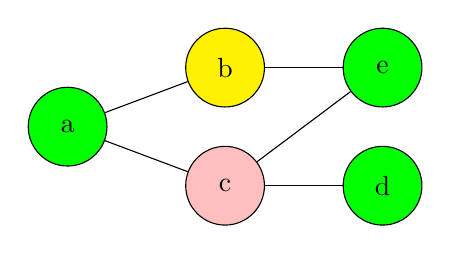
\begin{tikzpicture}[
				every node/.style={draw,circle},
				minimum size=10mm,
				node distance=2cm
			]
			\node[fill=green] (a) at (0,0) {a};
			\node[fill=yellow] (b) at (2cm,0.75cm) {b};
			\node[fill=pink] (c) at (2cm,-0.75cm) {c};
			\node[fill=green, right of=c] (d) {d};
			\node[fill=green, right of=b] (e) {e};
			\draw (a) -- (b);
			\draw (b) -- (e);
			\draw (e) -- (c);
			\draw (c) -- (d);
			\draw (a) -- (c);
		\end{tikzpicture}
	\]
	Ci sono poi molte varianti sul tema. I nodi possono avere delle proprietà, come il colore (in questo esempio) o la forma. Gli archi possono avere o no delle frecce.
\end{frame}

\begin{frame}{Esempio di quantificazione universale su grafi}
	\begin{columns}
		\column{0.35\textwidth}
		\[
			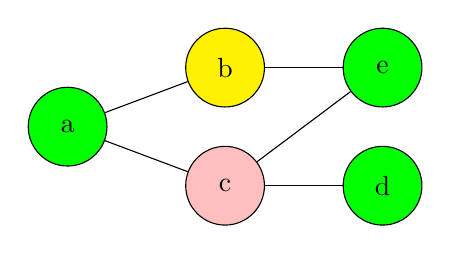
\begin{tikzpicture}[
					every node/.style={draw,circle},
					minimum size=10mm,
					node distance=2cm
				]
				\node[fill=green] (a) at (0,0) {a};
				\node[fill=yellow] (b) at (2cm,0.75cm) {b};
				\node[fill=pink] (c) at (2cm,-0.75cm) {c};
				\node[fill=green, right of=c] (d) {d};
				\node[fill=green, right of=b] (e) {e};
				\draw (a) -- (b);
				\draw (b) -- (e);
				\draw (e) -- (c);
				\draw (c) -- (d);
				\draw (a) -- (c);
			\end{tikzpicture}
		\]
		\column{0.6\textwidth}

		Vogliamo verificare che
		\begin{itemize}
			\item \prop{Tutti i nodi connessi con c sono verdi}
		\end{itemize}
		ovvero
		\begin{itemize}
			\item \prop{Per ogni $x$, se $x$ è connesso con c allora $x$ è verde}
		\end{itemize}
		è vera (l'universo del discorso sono i nodi del grafo).

		\medskip Si vede facilmente che tutte queste sono vere:
		\begin{itemize}
			\item $x \mapsto a$: \prop{se a è connesso con c allora a è verde};
			\item $x \mapsto b$: \prop{se b è connesso con c allora b è verde};
			\item $x \mapsto c$: \prop{se c è connesso con c allora c è verde};
			\item $x \mapsto d$: \prop{se d è connesso con c allora d è verde};
			\item $x \mapsto e$: \prop{se e è connesso con c allora e è verde}.
		\end{itemize}
	\end{columns}
\end{frame}

\begin{frame}{Quantificatore esistenziale (1)}
	\begin{columns}
		\column{0.35\textwidth}
		\[
			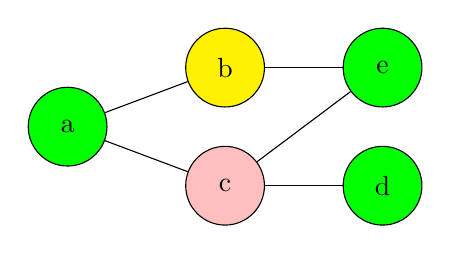
\begin{tikzpicture}[
					every node/.style={draw,circle},
					minimum size=10mm,
					node distance=2cm
				]
				\node[fill=green] (a) at (0,0) {a};
				\node[fill=yellow] (b) at (2cm,0.75cm) {b};
				\node[fill=pink] (c) at (2cm,-0.75cm) {c};
				\node[fill=green, right of=c] (d) {d};
				\node[fill=green, right of=b] (e) {e};
				\draw (a) -- (b);
				\draw (b) -- (e);
				\draw (e) -- (c);
				\draw (c) -- (d);
				\draw (a) -- (c);
			\end{tikzpicture}
		\]
		\column{0.6\textwidth}

		La proposizione
		\begin{proposition}
			Esiste $x$ tale che \ldots
		\end{proposition}
		è vera se esiste almeno un valore dell'universo del discorso che possiamo rimpiazzare in $x$ per rendere vera la proposizione nei $\ldots$

		\medskip
		Ad esempio, nel grafo di prima, la proposizione
		\begin{proposition}
			Esiste almeno un nodo verde connesso con b
		\end{proposition}
		ovvero
		\begin{proposition}
			Esiste $x$ tale che $x$ è verde ed $x$ è connesso con b
		\end{proposition}
		è vera, basta prendere come \alert{esempio} la sostituzione $x \mapsto a$.
	\end{columns}
\end{frame}

\begin{frame}{Quantificatore esistenziale (2)}
	\begin{columns}
		\column{0.35\textwidth}
		\[
			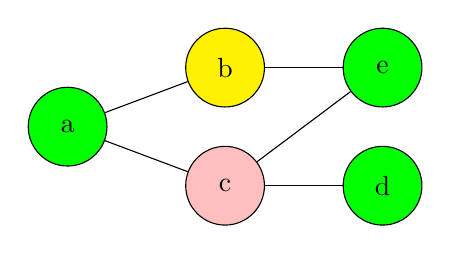
\begin{tikzpicture}[
					every node/.style={draw,circle},
					minimum size=10mm,
					node distance=2cm
				]
				\node[fill=green] (a) at (0,0) {a};
				\node[fill=yellow] (b) at (2cm,0.75cm) {b};
				\node[fill=pink] (c) at (2cm,-0.75cm) {c};
				\node[fill=green, right of=c] (d) {d};
				\node[fill=green, right of=b] (e) {e};
				\draw (a) -- (b);
				\draw (b) -- (e);
				\draw (e) -- (c);
				\draw (c) -- (d);
				\draw (a) -- (c);
			\end{tikzpicture}
		\]
		\column{0.6\textwidth}

		Vediamo invece la proposizione
		\begin{proposition}
			Esiste $x$ tale che $x$ è rosa e $x$ è connesso con b
		\end{proposition}
		Questa proposizione è falsa: rimpiazzando $x$ con un nodo si ottengono sempre proposizioni false:
		\begin{itemize}
			\item $x \mapsto a$: \prop{a è rosa e a è connesso con b}
			\item $x \mapsto b$: \prop{b è rosa e b è connesso con b}
			\item $x \mapsto c$: \prop{c è rosa e c è connesso con b}
			\item $x \mapsto d$: \prop{d è rosa e d è connesso con b}
			\item $x \mapsto e$: \prop{e è rosa e e è connesso con b}
		\end{itemize}
	\end{columns}
\end{frame}

\begin{frame}{Più quantificatori (1)}
	Consideriamo la proposizione
	\begin{proposition}
		Ogni nodo verde è connesso con almeno un nodo giallo.
	\end{proposition}
	Usando le forme standard ``\emph{per ogni}\,'' ed ``\emph{esiste \ldots tale che}\,'' abbiamo
	\begin{proposition}
		Per ogni x, se x è verde esiste y tale che y è giallo e x è connesso con y.
	\end{proposition}
	Per determinare se è vera, proviamo a sostituire ad $x$, tutti i possibili nodi, e otteniamo:
	\begin{itemize}
		\item $x \mapsto a$: \prop{se a è verde esiste y tale che y è giallo ed a è connesso con y}
		\item $x \mapsto b$: \prop{se b è verde esiste y tale che y è giallo e b è connesso con y}
		\item $x \mapsto c$: \prop{se c è verde esiste y tale che y è giallo e c è connesso con y}
		\item $x \mapsto d$: \prop{se d è verde esiste y tale che y è giallo e d è connesso con y}
		\item $x \mapsto e$: \prop{se e è verde esiste y tale che y è giallo ed e è connesso con y}
	\end{itemize}
	Verifichiamole una alla volta.
\end{frame}

\begin{frame}{Più quantificatori (2)}
	\begin{itemize}
		\item ``\prop{se a è verde esiste y tale che y è giallo ed a è connesso con y}'' è vera perché:\\
		      \begin{itemize}
			      \item ``\prop{a è verde}'' è vera
			      \item ``\prop{esiste y tale che y è giallo ed a è connesso con y}'' è vera, perché c'è l'esempio:
			            \begin{itemize}
				            \item $y \mapsto b$: ``\prop{b è giallo ed a è connesso con b}'' che è vera
			            \end{itemize}
			      \item quindi l'implicazione è vera;
		      \end{itemize}
		\item ``\prop{se b è verde esiste y tale che y è giallo e b è connesso con y}'' è vera perché:
		      \begin{itemize}
			      \item ``\prop{b è verde}'' è falsa;
			      \item quindi l'implicazione è vera, anche senza andare a guardare il conseguente;
		      \end{itemize}
		\item ``\prop{se c è verde esiste y tale che y è giallo e c è connesso con y}'' è vera come per a;
		\item ``\prop{se d è verde esiste y tale che y è giallo e d è connesso con y}'' è falsa perché:
		      \begin{itemize}
			      \item ``\prop{d è verde}'' è vera;
			      \item ``\prop{esiste y tale che y è giallo ed a è connesso con y}'' è falsa perché:
			            \begin{itemize}
				            \item $y \mapsto a$: \prop{a è giallo ed a è connesso con a}'' è falsa;
				            \item $y \mapsto b$: \prop{b è giallo ed a è connesso con b}'' è falsa;
				            \item \ldots in maniera analoga le altre
			            \end{itemize}
			      \item quindi l'implicazione è falsa;
		      \end{itemize}
	\end{itemize}
\end{frame}

\begin{frame}{Più quantificatori (3)}
	Otteniamo così che la sostituzione $x \mapsto d$ dà origine ad un controesempio
	\begin{proposition}
		se d è verde esiste y tale che y è giallo e d è connesso con y
	\end{proposition}
	che è falso, quindi la proposizione originaria
	\begin{proposition}
		Per ogni x, se x è verde esiste y tale che y è giallo e x è connesso con y
	\end{proposition}
	è falsa.

	\medskip
	Ovviamente, se ci accorgiamo a colpo d'occhio che $x \mapsto d$ è la sostituzione che crea problemi, possiamo provare subito quella invece di provare prima con $a$, $b$ e $c$.
\end{frame}

\begin{frame}{Esercizi consigliati}
	Esercizi da 2 a 8 del Capitolo 1. Esercizi da 1 a 4 del Capitolo 5.
\end{frame}

\end{document}